\section{Motivation}\label{sec:motiv}

Methods based on formal knowledge pay off almost exclusively at large scales due to the high level of theoretical understanding and practical investment that they require from both developers and users.
But for the same reason, it is difficult for individual approaches to reach those large scales.
Today's successful projects such as the Mizar Mathematical Library \cite{mizar}
%verification of the L4 microkernel \cite{l4verified}
or the formal proof of the Kepler conjecture \cite{flyspeck}
are built on double-digit person years of investment.

Therefore, the last few decades have seen increasing specialization into \textbf{isolated, mutually incompatible systems} and \textbf{incompatible overlapping libraries of formal knowledge}.
Moreover, during that time the advances in computer and internet technology have dramatically changed our expectations regarding scalability.
Many requirements have become critical that are not anticipated in the designs of formal systems such as collaboration, system interoperability, and modularity.
\textbf{Three central design choices have proved problematic}:

{\bf Fixed Foundations}
Virtually all current systems are based on a fixed foundation, i.e., a fixed logic in which all formalizations in that system are stated.
While the vast majority of classical mathematics has been formulated in axiomatic set theory, alternative foundations such as higher-order logic or constructive type theory have become important in computer-supported approaches.
Today almost all systems use foundations that are different from each other and different from classical set theory, and all attempts to find the ``mother of all logical systems'' (and convince others to use it) have failed, e.g., the qed project \cite{qed}.
This is all the more frustrating because these incompatibilities are often irrelevant for high-level formalization goals.
  
{\bf Homogeneity}
Classical mathematics uses the heterogeneous method, going back to the works by Bourbaki \cite{bourbakiunivers}, which focuses on defining \emph{theories} and stating every result in the smallest possible theory.
This allows using \emph{theory morphisms} to move results between theories in a truth-preserving way \cite{littletheories}.
Consequently, mathematics is usually carried out in highly abstracted settings where the foundational details are hidden.
Yet, virtually all formalizations in current systems are based on the homogeneous method, which uses only conservative extensions (e.g., definitions, theorems) of the fixed foundation to model mathematical knowledge.
Therefore, formalizations inherently depend on the fixed foundation.
%The combination of fixed foundation and homogeneous method means that a lot of -- expensive -- formalization work is needed just to build the mathematical setting of interest (e.g., the real numbers) as a conservative extension of the fixed foundation.
%However, the resulting formalizations are actually less valuable: It becomes virtually impossible to move them between foundations.
%Therefore, almost all current systems are mutually incompatible, with only a few hand-crafted translations between them (e.g., \cite{hol_coq,isahol_isazf}).

{\bf Local Scale} Mathematical research and applications are distributed globally, and mathematical knowledge is highly interlinked by explicit and implicit references.
Therefore, a computer-supported management system should support global interlinking, and management algorithms have to scale up to large (global) data sets.
Yet, virtually all current systems operate under the implicit assumption that all knowledge is locally available and loaded into main memory.
In fact, because these systems have initially focused on soundness and efficiency at small scales, large scale knowledge management has proved very difficult to add as an afterthought, often prohibitively so.
%many are designed in such a way that every run of the system verifies not only the theorem at hand but every single theorem leading up to it.
\medskip

However, \textbf{developers' resources are stretched thin already} by developing (and maintaining) their system at all.
Therefore, the gradual migration towards new designs that overcome these problems is extremely difficult.

The {\mmt} language and system have been designed from scratch to provide a uniform solution to the above three problems: \textbf{\mmt is a globally scalable Module system for Mathematical Theories that abstracts from and mediates between different foundations and maximizes the reuse of concepts, tools, and formalizations}.
Thus, it provides a theoretical and practical foundation for formal knowledge in the large.

\section{The \mmt Language}

\mmt is systematically \textbf{foundation-independent}.
It separates large scale concerns, which are addressed generically by {\mmt}, and small scale concerns, which are addressed by individual foundational languages.
Thus, foundation-specific development can focus on the logical core of the foundation instead of spending resources on ad hoc large scale support.
Dually, large scale support can be developed generically (and often more easily) at the {\mmt} level.

\mmt \textbf{integrates successful representational paradigms}
\begin{compactitem}
\item the logics-as-theories representation from proof theoretical frameworks like LF \cite{lf},
\item categories of theories from model theoretical frameworks like institutions \cite{institutions},
\item the structured theories from algebraic specification languages like \cite{asl},
\item reuse along theory morphisms from the ``little theories'' approach \cite{littletheories},
%\item declarations of constants and named realizations from type theory,
\item the Curry-Howard correspondence from type/proof theory \cite{curry,howard},
\item URIs as logical namespace identifiers from {\openmath} \cite{openmath},
\item standardized XML-based interchange syntax from markup languages like {\omdoc} \cite{omdoc}
\end{compactitem}
and makes them available in a single, coherent representational system for the first time.
The combination of these features is \textbf{based on a small set of carefully chosen, orthogonal primitives} in order to obtain a simple and extensible language design.
%In particular, {\mmt} coherently realizes two goals that are often mutually exclusive in knowledge representation languages:
%\begin{inparaenum}[(i)]
% \item the automation potential offered by machine-understandable representations, as pursued for example in proof assistants
% \item the universal applicability offered by a generic meta-language, as pursued in XML-based content markup languages.
%\end{inparaenum}
%Being a foundationally unconstrained language with a precise semantics

The central concept of \mmt is that of a \textbf{theory}, which is a named list of declarations.
Most importantly, the declaration of a \textbf{constant} introduces a new name possibly with additional attributes such as type, definiens, or notation.
Relative to a theory, \textbf{objects} are formed as syntax trees with binding.

These three concepts are sufficient to naturally represent virtually all formal languages.
\begin{compactitem}
\item All languages are represented uniformly as {\mmt} theories.
This includes foundations, logical frameworks, logics and type theories, signatures and theories, set theories.
\item All operators and symbols of a language are represented as \mmt constants.
This includes the sort, constant, function, and predicate symbols of logics, the base type, type operators, and term constructors of type theories, the concepts, relations, and individuals of ontologies, as well as -- via the Curry-Howard correspondence -- the judgments, inference rules, axioms, and theorems of calculi.
\item All composed expressions are represented as objects.
This includes formulas, derivations and proofs, terms, types, kinds, and universes, etc.
\end{compactitem}

All {\mmt} theories are related via \textbf{theory morphisms}, which are used to uniformly describe representation theorems between theories.
These include translations, functorial representations, implementations, and models.
They are also used as the semantics of \textbf{import} declarations within theories, which uniformly represent all aspects of building theories modularly.
These include inheritance and instantiation.

\begin{wrapfigure}r{6cm}
\vspace{-1em}
\begin{tikzpicture}[xscale=.95]
\node (A) at (0,3)  {$\cn{LF}$};
\node (A') at (2,3)  {$\cn{LF}+X$};
\node (C) at (-1,1.5)   {$\cn{FOL}$};
\node (C') at (1,1.5) {$\cn{HOL}$};
\node (E) at (-3,0) {$\cn{Monoid}$};
\node (E') at (1,0)  {$\cn{Ring}$};
\draw[dotted,arrow](A) -- (C);
\draw[dotted,arrow](A) -- (C');
\draw[dotted,arrow](C) -- (E);
\draw[dotted,arrow](C) -- (E');
\draw[dashed,arrow](A) --node[above] {$m$} (A');
\draw[arrow](C) --node[above] {$m'$} (C');
\draw[dashed,arrow](E) to[out=-30,in=-150] node[above] {$\cn{add}$} (E');
\draw[dashed,arrow](E) to[out=30,in=150] node[below] {$\cn{mult}$} (E');
\end{tikzpicture}
\end{wrapfigure}

A key innovation of {\mmt} is the \textbf{meta-theory} relation between theories.
Let us write $M/T$ to express that we work in the object language $T$ using the meta-language $M$.
For example, most of mathematics is carried out in $\cn{FOL}/\cn{ZFC}$, i.e., first-order logic is the meta-language, in which set theory is defined.
$\cn{FOL}$ itself might be defined in a logical framework such as $LF$~\cite{lf}, and within $ZFC$, we can define the language of natural numbers, which yields $\cn{LF}/\cn{FOL}/\cn{ZFC}/\cn{Nat}$.

In {\mmt}, all of these languages are represented as theories, each of which may be reused as the meta-theory of another one.
Crucially, the meta-theory indicates both to humans and to machines how a theory is to be understood.
For example, interpretations of $\cn{ZFC}$ must understand $\cn{FOL}$, and the typing relation of $\cn{FOL}$ is inherited from $\cn{LF}$.
The diagram of \mmt theories on the right gives an example.
Here dotted arrows denote the meta-theory relations, solid arrows are language translations, and dashed arrows are imports.
$\cn{LF}+X$ represents any extension of LF with additional features.

We can see {\mmt} as the \textbf{last step in a progression towards more abstract formalisms} as indicated below.
In conventional mathematics, domain knowledge is expressed directly in ad hoc notation.
Logic provided a formal syntax and semantics for this notation.
Logical frameworks provided a formal way to define this syntax and semantics.
Now {\mmt} adds a meta-level, at which we can design logical frameworks.
That makes {\mmt} very robust against future language developments: We can develop $\cn{LF}+X$ without any change to the {\mmt} infrastructure and can easily migrate all results obtained within LF.

\begin{center}
\begin{tabular}{|l|l|l|l|}
\hline
Mathematics      & Logic            & Logical Frameworks & Foundation-Independence \\
\hline
%natural language & natural language & natural language & natural language \\
                 &                  &                  & {\mmt}\\
                 &                  & logical framework & logical framework\\
                 & logic            & logic            & logic\\
domain knowledge & domain knowledge & domain knowledge & domain knowledge \\
\hline
\end{tabular}
\end{center}

\cite{RK:mmt:10} provides a comprehensive (albeit by now slightly outdated) introduction to the \mmt language.
A more recent treatment that focuses on the representation of logics in \mmt is given in \cite{rabe:howto:14}.

%%%%%%%%%%%%%%%%%%%%%%%%%%%%%%%%%%%%%%%%%%%%%%%%%%%%%%%%%%%
\section{The \mmt System}\label{sec:mmtsys}

\begin{figure}[htb]
\begin{center}
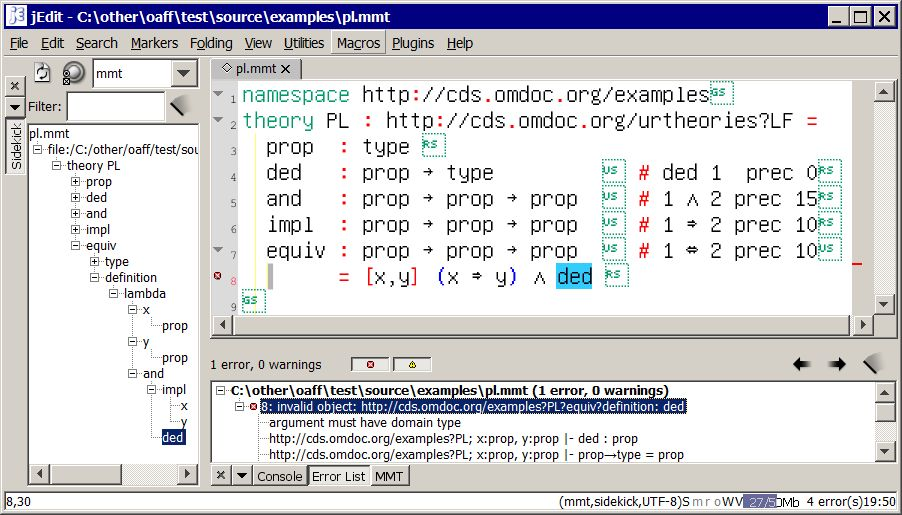
\includegraphics[width=\textwidth]{img/jedit-sidebar-errors.jpg}
\end{center}
\caption{\mmt IDE based on jEdit}\label{fig:jedit}
\end{figure}

\begin{figure}[htb]
\begin{center}
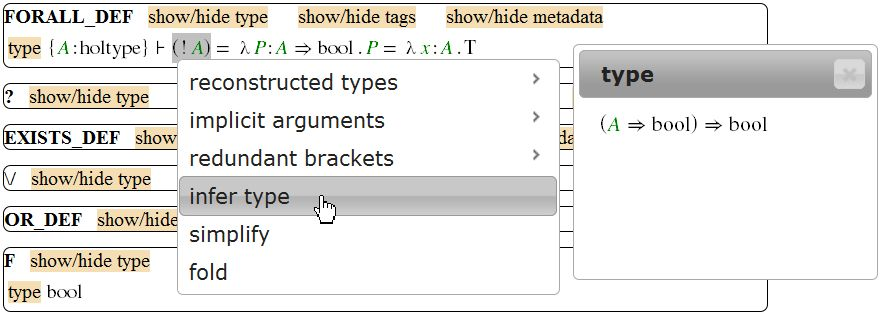
\includegraphics[width=\textwidth]{img/type-inference.jpg}
\end{center}
\caption{Type Inference in the \mmt Web Server}\label{fig:web}
\end{figure}

Exploiting the small number of primitives in the {\mmt} language, the {\mmt} API provides a simple scalable implementation of {\mmt} and {\mmt}-based functionality (written in the functional and object-oriented language Scala \cite{scala}).

Due to the generality of \mmt, one might think that it is not possible to implement deep, meaningful functionality at the \mmt level.
Indeed, implementing any result requires first generalizing it to the \mmt level.
However, \textbf{practical experience has shown that most results can be generalized to the \mmt level}.
For each result, this may require a substantial research effort, which samples existing results for specific foundations and recovers them as special cases of a general principle.
But it is doubly rewarding: Besides yielding a general result, the abstract level of \mmt provides a more focused view on a concept and often yields clearer intuitions.

All \mmt-level functionality is implemented foundation-independently, and foundation-specific aspects (if any) are left abstract and supplied by plugins.
Crucially, experience shows that the vast \textbf{majority of the implementation is foundation-independent}.
For example, the \mmt API comprises $>30,000$ lines of code, and the LF plugin, which provides in particular typing and proof rules for LF, comprises $<2000$ lines.
\medskip

\textbf{Logical results implemented at the \mmt level} include notations and parsing, module system and theory transformations, type reconstruction and simplification, as well as a (so far very basic) theorem prover.
For example, the foundation-independent aspects of type reconstruction include lookup of identifiers, implicit arguments, solving for meta-variables, constraint delay, and error reporting.
The LF plugin only supplies $\sim 10$ rules of a few lines each, which correspond directly to the statement of the rules on paper -- advanced aspects such as modularity and unsolved meta-variables remain transparent to the plugin developer.
\medskip

\textbf{Knowledge management results implemented at the \mmt level} include project management, build system, IDE (build by integrating \mmt with the jEdit text editor), interactive browsing using HTML+presentation MathML \cite{mathml} and JavaScript, change management, as well as indexing, querying, and search (the latter builds on top of MathWebSearch \cite{mathwebsearch}).
Plugin interfaces allow the convenient import/export of content in other formats.

\mmt URIs serve as identifiers throughout the implementation and abstract from physical storage units such as file systems or versioned repositories.
\mmt maintains a catalog that maps URIs to physical locations.
\mmt content is loaded into memory only when needed, and the distribution of content over physical storage and networks remains transparent to \mmt-based services.

For example, Fig.~\ref{fig:jedit} shows screenshot of a definition of propositional logic with meta-theory LF in the \mmt IDE.
An intentionally introduced error was detected by type reconstruction and highlighted.
Note how the sidebar shows the abstract syntax tree of the theory: The types of the variables $x$ and $y$ were inferred and are displayed in the syntax tree even though type reconstruction for the whole object failed.
Other features include hyperlinks, context-sensitive auto-completion, or interactively solving for subexpressions based on the expected type.

Fig.~\ref{fig:web} shows a screenshot of a part of the {\mmt} web server.
It shows a fragment of the HOL Light library as imported into \mmt in \cite{KR:hollight:14}.
It shows how the web browser infers and displays the type of the selected subexpression (in the definition of the universal quantifier, which is written $!$ in HOL Light).
Other interactive features include folding subexpressions, hiding/showing inferred types, implicit arguments, and redundant brackets, or retrieving the definition of a symbol.
It is also 
%The selected declaration derives the rule $\frac{A,B\vdash C}{\vdash A\, imp\, (B\,imp\, C)}$ in the theory $\mathrm{IMP}$ of the implication connective $\mathrm{imp}$.
%Via the JOBAD context menu, the user called type inference on the selected subobject, which resulted in a dialog displaying the dynamically inferred type.

All this \textbf{functionality can be made available to individual formal systems at small cost} -- all foundation-specific code for the above two examples is contained in the LF plugin.
\medskip

Many features of the \mmt system are described in individual publications.
An overview is given in \cite{rabe:mmtabs:13}.
Source code, binaries, and documentation of the \mmt system are available at \url{http://uniformal.github.io}.

\section{Integrating Languages: The LATIN Atlas}\label{sec:atlas}

\begin{figure}[hbp]
\begin{center}
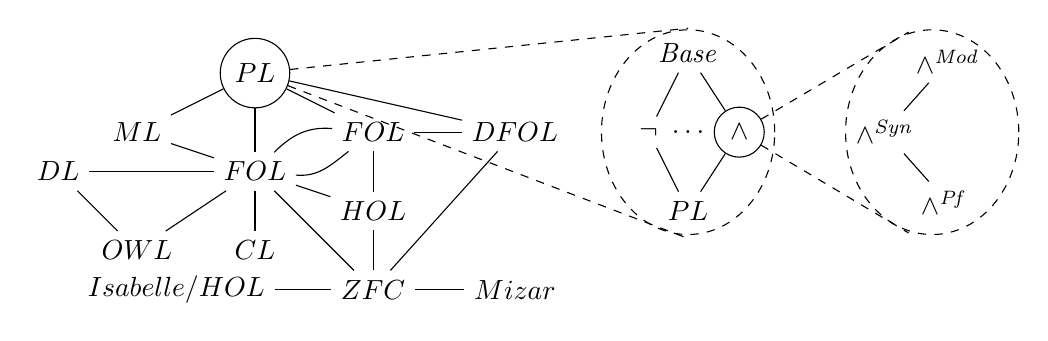
\begin{tikzpicture}
%The Logic Atlas
\node[circle,draw] (P)  at (4,4.25)   {$\cn{PL}$};
\node (M)  at (2.5,3.5) {$\cn{ML}$};
\node (S)  at (5.5,3.5) {$\cn{FOL}$};
\node (D)  at (7.3,3.5)   {$\cn{DFOL}$};
\node (F)  at (4,3)   {$\cn{FOL}$};
\node (C)  at (4,2)   {$\cn{CL}$};
\node (DL) at (1.5,3)   {$\cn{DL}$};
%\node (LL) at (1,3.5)   {$\cn{LL$};
\node (H)  at (5.5,2.5)   {$\cn{HOL}$};
\node (O)  at (2.5,2)   {$\cn{OWL}$};
\node (Mz) at (7.3,1.5)   {$\cn{Mizar}$};
\node (Z)  at (5.5,1.5)   {$\cn{ZFC}$};
\node (I)  at (3,1.5)   {$\cn{Isabelle/HOL}$};

\draw[\arrowtipmono-\arrowtip] (P) -- (F);
\draw[\arrowtipmono-\arrowtip] (P) -- (M);
\draw[\arrowtipmono-\arrowtip] (P) -- (S);
\draw[\arrowtipmono-\arrowtip] (P) -- (D);

\draw[-\arrowtip] (F)  -- (H);
\draw[-\arrowtip] (F)  -- (C);
\draw[-\arrowtip] (M)  -- (F);
\draw[-\arrowtip] (DL) -- (F);
\draw[-\arrowtip] (S)  -- (D);
\draw[-\arrowtip] (S)  -- (H);
\draw[-\arrowtip] (DL) -- (O);
\draw[-\arrowtip] (O)  -- (F);
\draw[-\arrowtip] (F) to[out=45,in=175] (S);
\draw[-\arrowtip] (S) to[out=218,in=-5]  (F);
\draw[-\arrowtip] (H)  -- (Z);
\draw[-\arrowtip] (D)  -- (Z);
\draw[-\arrowtip] (Z)  -- (Mz);
\draw[-\arrowtip] (I)  -- (Z);
\draw[\arrowtipmono-\arrowtip] (F) -- (Z);

%PL details with base, negation and conjunction
\node (B) at (9.5,4.5) {$\mathit{Base}$};
\node (N) at (9,3.5) {$\neg$};
\node (L) at (9.5,3.5) {$\ldots$};
\node[circle,draw] (A) at (10.15,3.5) {$\wedge$};
\node (PL) at (9.5,2.5) {$\cn{PL}$};
\draw[\arrowtipmono-\arrowtip] (B) -- (N);
\draw[\arrowtipmono-\arrowtip] (B) -- (A);
\draw[\arrowtipmono-\arrowtip] (N) -- (PL);
\draw[\arrowtipmono-\arrowtip] (A) -- (PL);
\draw[dashed] (9.5,3.5) ellipse (1.1cm and 1.3cm);
\draw[-,dashed] (P) -- (9.5,2.15);
\draw[-,dashed] (P) -- (9.5,4.82);

%Syn, Pf, Mod span for Conjunction
\node (AM) at (12.8,4.4)   {$\wedge^{\mathit{Mod}}$};
\node (AS) at (12,3.5) {$\wedge^{\mathit{Syn}}$};
\node (AP) at (12.8,2.6)   {$\wedge^{\mathit{Pf\,\,}}$};
\draw[\arrowtipmono-\arrowtip] (AS) -- (AP);
\draw[-\arrowtip] (AS) -- (AM);
\draw[dashed] (12.6,3.5) ellipse (1.1cm and 1.3cm);
\draw[-,dashed] (A) -- (12.3,4.77);
\draw[-,dashed] (A) -- (12.3,2.22);
\end{tikzpicture}
\end{center}
\caption{A Fragment of the LATIN Atlas}\label{fig:atlas}
\end{figure}

The LATIN project \cite{CHKMR:latinabs:11,project:latin} (2009-2012) built a \textbf{library of formalizations of logics and related languages} as well as translations between them.
It used LF as the meta-theory for all languages.

Fig.~\ref{fig:atlas} shows a high-level view of a fragment of the resulting diagram of \mmt theories.
The left side shows some of the logics, the middle zooms into the modular definition of propositional logic, and the right side zooms in further to show the definition of conjunction as a triple of syntax, proof theory, and model theory.

The formalized \textbf{logics} include propositional, first-order, sorted first-order, common, higher-order, modal, description, and linear logics.
Type theoretical features, which can be freely combined with logical features, include the $\lambda$-cube, product and union types, as well as base types like booleans or natural number.
In many cases alternative formalizations are given (and related to each other), e.g., Curry- and Church-style typing, or Andrews and Prawitz-style higher-order logic.
The logic \textbf{morphisms} include the relativization translations from modal, description, and sorted first-order logic to unsorted first-order logic,
%the interpretation of type theory in set theory,
the negative translation from classical to intuitionistic logic, and the translation from first to sorted first- and higher-order logic.
The model theoretical semantics is represented as theory morphisms from a logic into a theory representing a foundation.
The \textbf{foundations} include Zermelo-Fraenkel set theory, Church's higher-order logic, and Mizar's formalized set theory \cite{mizar}.

All representations systematically exploit modularity and form a single \textbf{highly interconnected diagram of \mmt theories}.
Every logical principle, e.g., as conjunction, the universal quantifier of first-order logic, or the extensionality principle of higher-order logic, is formalized in a separate module.
Thus, \textbf{logics can be composed modularly} from the individual features using the {\mmt} module system.
For example, logic of Isabelle \cite{isabelle} can be obtained by combining the modules for Church-style typing, simple function types, a boolean type, implication, typed universal quantification, and typed equality, as well as corresponding theories for the proof theory and corresponding theory morphisms for the model theory.

The full LATIN graph comprises several hundred modules and is available at \url{img/latin-graph.html}\footnote{absolute path: \url{http://uniformal.github.io/doc/philosophy/articles/img/latin-graph.html}} and spreads about 200 files.
Particularly interesting representations are described in detail in \cite{IR:foundations:10,HR:folsound:10,BRS:tptphol:08}.
The theoretical background of representing the proof and model theory of logics in \mmt is discussed in \cite{rabe:combining:10,rabe:howto:14}.

%\begin{wrapfigure}{r}{3cm}
%\vspace{-1em}
%\begin{tikzpicture}	
%\node (S) at (0,0) {$L^{Syn}$};
%%\node (B) at (-2.5,0) {$Base$};
%\node (P) at (1,1.3) {$L^{Pf}$};
%\node (M) at (1,-1.3) {$L^{Mod}$};
%\node (Z) at (1,-2.3) {$\mathcal{F}$};
%\draw[-\arrowtip](S) --node[near end,left] {$L^{mod}$} (M);
%\draw[right hook-\arrowtip](S) --node[near end,left] {$L^{pf}$} (P);
%\draw[-\arrowtip](M) .. controls (.7,-1.8) .. node[left] {$M$} (Z);
%\draw[\arrowtipmono-\arrowtip](Z) -- (M);
%%\draw[\arrowtipmono-\arrowtip] (B) --node[above] {$L^{truth}$} (S);
%\draw[-\arrowtip] (P) --node[right] {$L^{sound}$} (M);
%\end{tikzpicture}
%\vspace{-3em}
%\end{wrapfigure}
%
%All logics are represented following the $\LFI$ framework, i.e., they are represented as spans of LF theories including syntax, proof theory, and model theory.
%Similarly, the library includes various translations between these formal systems, many of which are logic translations in the sense of the $\LFI$ framework.
%
%Logic representations formalize the syntax, proof theory, and model theory of a logic as separate theories as indicated on the right.
%The syntax of a logic $L$ is represented as a theory $L^{Syn}$, which is then extended with the representation of proof rules to represent the proof theory as $L^{pf}$.
%The model theory of the logic is represented as a theory $L^{Mod}$ as an extension of the representation $\mathcal{F}$ of a foundation of mathematics.
%Then individual models are represented as theory morphisms $M$ into the foundation.
%Moreover, we can represent soundness proofs as a morphism $L^{sound}$ from the proof theory to the model theory of $L$.
%Similarly, logic translations are represented as triples of theory morphisms that formalize the translations of syntax, proof theory, and model theory.

\section{Integrating Libraries:\\ The Open Archive of Formalizations}

\begin{figure}[htb]
 \begin{center}
 \begin{tikzpicture}
% \node (MMT) at (3,1.5) {MMT};
 \node (L) at (2,1) {LF};
 \node (Lx) at (4,1) {LF+X};
% \draw[arrow](MMT) -- (L);
% \draw[arrow](MMT) -- (Lx);
 \draw[mono](L) -- (Lx);

 \draw[fill=red!60] (2,-.5) ellipse (3.2cm and .6cm);
 \node[color=red] at (-3.1,-.5) {LATIN logic library};
 \node at (2,-.7) {\ldots};

 \draw[fill=blue!60] (0,-2.25) ellipse (1.9cm and .8cm);

 \node (H) at (0,-.5) {HOL Light};
 \node[color=blue!80] at (-3.7,-2.25) {HOL Light library};
 \node (B) at (-1,-2) {Bool};
 \node (A) at (1,-2) {Arith};
 \node (E) at (0,-2.5) {\ldots};
 \draw[arrow](L) -- (H);
 \draw[arrow](H) -- (B);
 \draw[arrow](H) -- (A);
 \draw[arrow](B) -- (A);

 \draw[fill=olive] (4,-2.25) ellipse (1.9cm and .8cm);

 \node (M) at (4,-.5) {Mizar};
 \node[color=olive] at (7.3,-2.25) {Mizar library};
 \node (B') at (3,-2) {XBoole};
 \node (A') at (5,-2) {XReal};
 \node (E') at (4,-2.5) {\ldots};

 \node (A) at (1,-2) {Arith};
 \node (E) at (0,-2.5) {\ldots};
 \draw[arrow](L) -- (M);
 \draw[arrow](M) -- (B');
 \draw[arrow](M) -- (A');
 \draw[arrow](B') -- (A');
 \end{tikzpicture}
 \end{center}
\caption{Representing Libraries in \mmt}\label{fig:oaf}
\end{figure}

The OAF project \cite{project:oaf} (2014-2017) aims at \textbf{overcoming the isolation and mutual incompatibility between the various large libraries} of formal knowledge obtained by applying the homogeneous method to various fixed foundations such as Mizar \cite{mizar}, the HOL systems \cite{hol,isabellehol,hollight}, PVS \cite{pvs}, Coq and Matita \cite{coq,matita}, as well as the heterogeneous libraries of TPTP \cite{tptp} and IMPS \cite{imps}.
The project proceeds in $2$ phases, both of tremendous difficulty.
\medskip

In the first phase, we \textbf{make the existing libraries available in a standardized format} by importing them into \mmt.
This requires two steps for each library:
\begin{compactenum}
\item We represent the logic of the used system in \mmt relative to a logical framework.
This representation doubles as a documentation layer for the logic and often requires a deeper understanding of the logic and its implementation than published in the literature.
In some cases LF will be sufficient as a logical framework, but in other cases stronger logical frameworks may have to by designed within \mmt.
\item Much more difficultly, we implement exports from the used system into \mmt.
The specification of the export is relatively simple except when languages use very unusual idiosyncrasies.
But the difficulty of the implementation is huge and can even be impossible without refactoring the system.
Therefore, substantial collaboration from within the respective developer community is indispensable.
\end{compactenum}
At this point, these steps have been mostly completed for Mizar and HOL Light, resulting in the \mmt diagram of Fig.~\ref{fig:oaf}.
\medskip

In the second phase, we will be able to attack the \textbf{library integration problem}.
This problem cripples state-of-the-art integration attempts between homogeneous systems: Theorems about, for example, the real numbers defined in one foundation cannot be used to reason about the real numbers as defined in another foundation.
The heterogeneous method could avoid this problem because all formalizations could be moved easily along morphisms.
Therefore, an important goal is to refactor the existing libraries to be more heterogeneous and to investigate partial or approximate solutions.

A central method will be to use \textbf{interface logics and interface theories} akin to the use of interfaces in software engineering.
Every problem should be stated in the weakest possible interface logic and theory, and then individual foundations that realize the interface can be used to obtain the proof.
This is crucial because foundations are usually substantially more expressive than the interface logic needed to state a problem.
For example, axiomatic set theory, higher-order logic, and constructive type theory are common foundations, but we can give an interface theory for the real numbers in a much weaker logic, e.g., a fragment of second-order logic.
While giving a logic translation between any two typical foundations can be prohibitively difficult, a weak interface logic can be easily imported into all of them.
This is no coincidence: Whereas foundations are designed to be simple and logically very expressive (because they should be fixed and implemented once and for all), interface logics should be as inexpressive as possible even if that makes them more complex.

The LATIN logic library already developed most of the needed interface logics.
This will have to complemented with a library of interface theories for the typical domains of computer science and mathematics.

\begin{wrapfigure}r{4cm}\vspace*{-1em}
  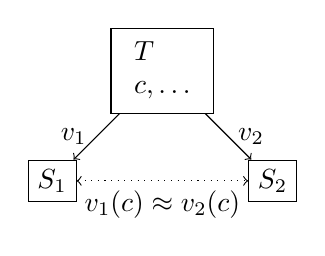
\begin{tikzpicture}[scale=1.4]
    \node[draw] (tg1) at (0,0) {$S_1$};
    \node[draw] (tg2) at (2,0) {$S_2$};
    \node[draw] (if) at (1,1) {$\begin{array}{l}{T}\\c,\ldots\end{array}$};
    \draw[->] (if) -- node[left]{$v_1$} (tg1);
    \draw[->] (if) -- node[right]{$v_2$} (tg2);
    \draw[dotted,<->] (tg1) --node[below]{$v_1(c)\approx v_2(c)$} (tg2);
  \end{tikzpicture}
  \vspace{-2em}
\end{wrapfigure}

Interfaces also provide a way to integrate libraries by using \textbf{alignments} \cite{RKS:integration:11}.
In the diagram on the right, an interface theory $T$ is realized by two systems $S_1$ and $S_2$, which is witnessed by two theory morphisms $v_i:T\to S_i$. For a $T$-symbol $c$, we say that $v_1(c)$ and $v_2(c)$ are \emph{aligned} via $(c,v_1,v_2)$.
Alignments provide a semantically backed concept for cross-references between libraries and provide a starting point for library translations that overcome the library integration problem.


%\section{System Integration}
%
% Hets, Twelf, Specware, filtering

%\citeByNumber{3d} and \citeByNumber{6} combine these two systems using {\mmt} an interlingua for system integration via its concrete syntax based on {\omdoc}.
%The benefit for LF/Twelf is that logics represented in LF can be (via Hets) easily connected to various interactive and automated theorem provers, model finders, model checkers, and conservativity checkers -- thus providing much more efficient proof support than mere proof checking.
%The benefit for institutions/Hets is that (via Twelf) logics are defined declaratively and their implementations derived uniformly instead of each logic being implemented ad hoc as a part of the Hets code base.
%Thus, the trustworthiness of the implementation of logics is increased, and correctness of logic translations can be mechanically verified.
%Moreover, the effort of adding new logics or translations to Hets is greatly reduced.
